\section{Linguaggi Regolari}
Un FA (NFA "[[Automi a Stati Finiti Non Deterministici]]" o DFA "[[Automi a Stati Finiti Non Deterministici]]) è un metodo per costruire una macchina che riconosce linguaggi regolari.\\
Un'\textit{espressione regolare} è un modo dichiarativo per descrivere un linguaggio regolare
Esempio: $$01* + 10*$$
Le espressioni regolari sono usate ad esempio in:
\begin{itemize}
	\item comandi UNIX (\textit{grep})
	\item strumenti per l'analisi lessicale di UNIX (\t{lex} \textit{Lexical analyzer generator}) e \t{flex} (\textit{Fast Lex})
	\item editor di testo
\end{itemize}
\subsection{Espressioni regolari}
sono costruite utilizzando:
\begin{itemize}
	\item un insieme di \textit{costanti} di base:
		\begin{itemize}
			\item $\epsilon$ per la stringa vuota
			\item $\varnothing$ per il linguaggio vuoto
			\item $a, b,...$ per i simboli $a,b,... \in \sum$
		\end{itemize}
	\item collegati da \textit{operatori}:
		\begin{itemize}
			\item $+$ per l'unione
			\item $.$ per la concatenazione
			\item $*$ per la chiusura di Kleene
		\end{itemize}
	\item Raggrupati usando le \textit{parentesi} $()$
\end{itemize}
Se $E$ è un espressione regolare, allora $L(E)$ è il \textit{linguaggio rappresentato da $E$}. La definizione di $L(E)$ è induttiva:
\begin{itemize}
	\item \g{Caso Base}:
		\begin{itemize}
			\item $L(\epsilon) = \{ \epsilon \}$
			\item $L(\varnothing) = \varnothing$
			\item $L(a) = \{a\}$
		\end{itemize}
	\item \g{Caso induttivo}:
		\begin{itemize}
			\item $L(E + F) = L(E) \cup L(F)$
			\item $L(EF) = L(E).L(F)$
			\item $L(E*) = L(E)^*$
			\item $L((E)) = L(E)$
		\end{itemize}
\end{itemize}
\g{Esempio}\\
$L=\{w \in \{0,1\}^* : 0$ e $1$ alternati in $w \}$\\
$(01)^* + (10)^* + 1(01)^* + 0(10)^*$ oppure $(\epsilon +1)(01)^*(\epsilon+0)$
\subsubsection{Precedenza}
Come per le espressioni aritmetiche, anche per le espressioni regolari ci sono delle \textit{regole di precedenza} degli operatori
\begin{enumerate}
	\item Chiusura di Kleene
	\item Concatenazione (punto)
	\item Unione
\end{enumerate}
\g{Esempio}\\
$01^*+1$ è raggruppato in $(0(1)^*)+1$\\
e denota un linguaggio \textit{diverso} da $(01)^*+1$
\subsection{Conversione per eliminazione di stati}
La procedura che vedremo è in grado di convertire un \textit{qualsiasi automa} (DFA o NFA) in un'{espressione regolare} equivalente.\\
Si procede per {eliminazione di stati}.\\
Quando uno stato $q$ viene eliminato i cammini che passano per $q$ scompaiono.\\
Si aggiungono nuove \textit{transizioni etichettate con espressioni regolari} che rappresentano i cammini eliminati.\\
Alla fine otteniamo un'espressione regolare che rappresenta \textit{tutti i cammini} dallo stato iniziale ad uno stato finale.\\
	$\rightarrow$ cioè il {linguaggio riconosciuto dall'automa}

\subsubsection{Da NFA a GNFA}
\mezzapagina
\begin{enumerate}
	\item Nuovo stato iniziale $q_{start}$ con transizione $\varepsilon$ verso il vecchio $q_0$ 
	\item Nuovo stato finale $q_{accept}$ con transizione $\varepsilon$ da tutti i vecchi stati finali $q\in F$ 
	\item Rimpiazzo transizioni multiple tra due stati con l'unione delle etichette
	\item Aggiungo transizioni etichettate con $\varnothing$ tra stati non collegati da transizioni
\end{enumerate}
\spazio
\begin{center}
	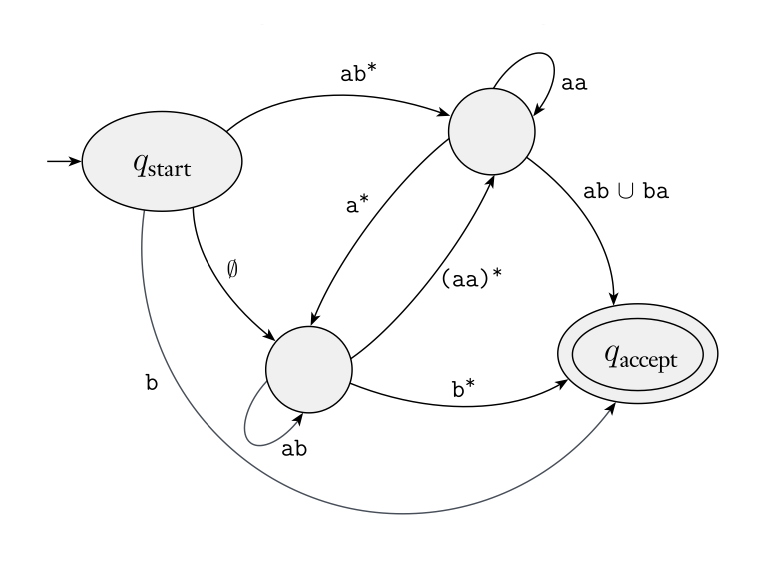
\includegraphics[scale=0.5]{img/NFAtoGNFA.png} 
\end{center}
\finemezzapagina
\subsection{Definizione formale di GNFA}
Un Automa a Stati Finiti Non Deterministico Generalizzato (GNFA) è una quintupla:
	$A=(Q, \sum, \delta, q_{start}, q_{accept})$
\begin{itemize}
	\item $Q$ è un insieme finito di \textit{stati}
	\item $\sum$ è un \textit{albero finito}
	\item $\delta : Q \backslash \{q_{accept}\} \times Q \backslash \mapsto R$ è una \textit{funzione di transizione} che prende in input \textit{2 stati} e restituisce 
		una \textit{espressione regolare} su $\sum$
	\item $q_{start} \in Q$ è lo \textit{stato iniziale}
	\item $q_{accept}$ è lo \textit{stato finale}
\end{itemize}
\subsubsection{Computazione di un GNFA}
Data una parola $w= w_1 w_2 ... w_m$ , dove $w_i \in \sum^*$
Una \textit{computazione} di un GNFA $A$ con input $w$ è una sequenza di stati $r_0r_1...r_m$ che rispetta \textit{2 condizioni}:
\begin{enumerate}
	\item $r_0 = q_{start}$ (inizia dallo stato iniziale)
	\item Per ogni $i, w_i \in L(R_i), dove R_i = \delta(r_{i-1}, r_i)$ (\textit{rispetta la funzione di transizione})
\end{enumerate}
Una computazione \textit{accetta} la parola $w$ se \textit{termina nello stato finale} ($r_m = q_{accept}$)\\\\
\mezzapagina
\begin{itemize}
	\item Partiamo da un GNFA con $k$ stati, dove $k\geq 2$ 
	\item Se $k>2$, eliminiamo uno stato $q_{rip}$ per ottenere un GNFA con $k-1$ stati.
	\item Quandk $k=2$, l'etichetta della transiione da $q_{start}$ a $q_{accept}$ è l'espressione regolare equivalente.
\end{itemize}
\spazio
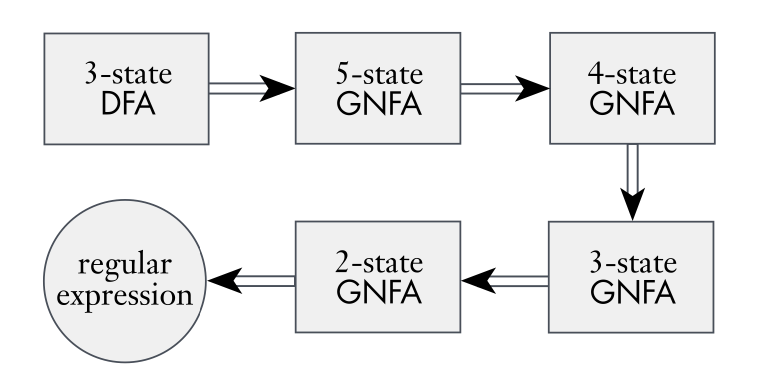
\includegraphics[scale=0.5]{img/GNFA_1.png}
\finemezzapagina

\mezzapagina
\begin{center}
	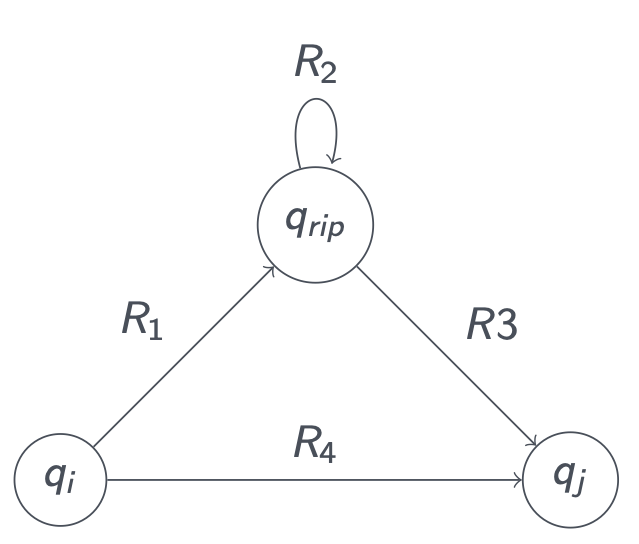
\includegraphics[scale=0.5]{img/GNFA_2.png}
\end{center}
\spazio
Se, nel GNFA:
\begin{enumerate}
	\item $q_i$ va in $q_{rip}$ con etichetta $R_1$ 
	\item $q_{rip}$ ha un self loop con etichetta $R_2$ 
	\item $q_{rip}$ va in $q_j$ con etichetta $R_3$ 
	\item $q_i$ va in $q_j$ con etichetta $R_4$ 
\end{enumerate}
\finemezzapagina

\mezzapagina
\begin{center}
	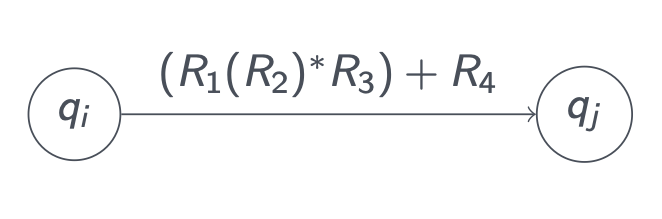
\includegraphics[scale=0.5]{img/GNFA_3.png}
\end{center}
\spazio
dopo l'eliminazione di $q_{rip}$, $q_i$ va in $q_j$ con etichetta 
$$(R_1(R-2)*R_3)+R_4$$
\finemezzapagina

\paragraph{Algoritmo di conversione}
\t{Convert(A)}
\begin{enumerate}
	\item Sia $k$ il numero di stati di $A$
	\item Se $k=2$, ritorna l'espressione $R$ che collega $q_{start}$ con $q_{accept}$
	\item Se $k > 2$, scegli $q_{rip} \in Q \backslash \{q_{start}, q_{accept}\}$ e costruisci un GNFA $A' = (Q',\sum, \delta ', q_{start}, q_{accept})$ come segue:
		\begin{itemize}
			\item $Q' = Q \backslash \{q_{rip}\}$
			\item per ogni $q_i \in Q' \backslash \{q_{accept}\}, q_j \in Q' \backslash \{q_{start}\}$, sia $\delta '(q_i,q_j) = (R_1(R_2)*R_3)+R_4$ 
		\end{itemize}
	 	 dove $R_1 = \delta (q_i,q_{rip}), R_2 = \delta (q_{rip}, q_{rip}), R_3 = \delta (q_{rip}, q_j)$ e $R_4=\delta (q_i, q_j)$
	 \item Ritorna il risultato calcolato da \t{Convert(A')}
\end{enumerate}

